\chapter{Methodology}
\label{ch:methods}

\section{Datasets}
\label{ch:datasets}
\label{sec:synthetic}\label{sec:hera}\label{sec:lofar}\label{sec:lofar_harder}
Three datasets were used in this work, summarised in \cref{fig:datasets}. The
LOFAR dataset\footcite{mesarcik2022,mesarcik2022data} is the most important,
because it is the only one made of real observations with labels checked by a
person; example images are shown in \cref{fig:lofar_overview}.

\begin{figure}[H]
  \centering
  \begin{tikzpicture}[
      font=\footnotesize,
      root/.style={draw, thick, rounded corners, fill=gray!15, align=center,
                   inner sep=5pt, font=\normalsize\bfseries},
      head/.style={draw, thick, rounded corners, align=center, inner sep=4pt,
                   text width=4.6cm, minimum height=1.1cm, font=\small\bfseries},
      info/.style={draw, rounded corners, align=left, inner sep=5pt,
                   text width=4.6cm, minimum height=4.6cm, anchor=north,
                   execute at begin node={\hyphenpenalty=10000}},
      edge/.style={thick, -{Stealth[length=2mm]}}]
    \node[root] (root) at (0,0) {Datasets};
    \node[head, fill=blue!10]   (syn)  at (-5.1,-1.6) {Synthetic\\[-1pt]{\footnotesize\mdseries generated by us}};
    \node[head, fill=orange!15] (hera) at ( 0.0,-1.6) {HERA\\[-1pt]{\footnotesize\mdseries simulated}};
    \node[head, fill=green!12]  (lof)  at ( 5.1,-1.6) {LOFAR\\[-1pt]{\footnotesize\mdseries real observations}};
    \foreach \n in {syn, hera, lof} \draw[edge] (root.south) -- (\n.north);
    \node[info] at ([yshift=-3mm]syn.south) {%
      Size: 1024$\times$265 px\\ (frequency $\times$ time)\\[2pt]
      1000 images\\
      Split: 700 train / 150 val / 150 test\\[2pt]
      RFI: 14.19\% of pixels\\[2pt]
      Labels: exact (RFI $>0.5\sigma$ of the noise)\\[2pt]
      Includes an instrument bandpass};
    \node[info] at ([yshift=-3mm]hera.south) {%
      Size: 512$\times$512 px\\[2pt]
      560 images (420 train / 140 test)\\
      After removing duplicates: 351 train / 135 test\\[2pt]
      RFI: 2.75\% of pixels\\[2pt]
      Labels: exact (simulated)\\[2pt]
      Too easy to compare methods ($F_1$ 0.9996); used only as a check};
    \node[info] at ([yshift=-3mm]lof.south) {%
      Size: 512$\times$512 px\\[2pt]
      7500 train / 109 test images\\
      After cleaning: 6621 train / 735 val / 109 test\\[2pt]
      RFI: 0.77\% of test pixels\\[2pt]
      Training labels: \aoflagger{}\\ ($F_1$ 0.57 against the expert)\\
      Test labels: human expert\\[2pt]
      Main dataset of this work};
  \end{tikzpicture}
  \caption[Summary of the three datasets]{Summary of the three datasets used
    in this work. ``val'' is the validation set used to choose checkpoints and
    thresholds.}
  \label{fig:datasets}
\end{figure}

\begin{figure}[H]
  \centering
  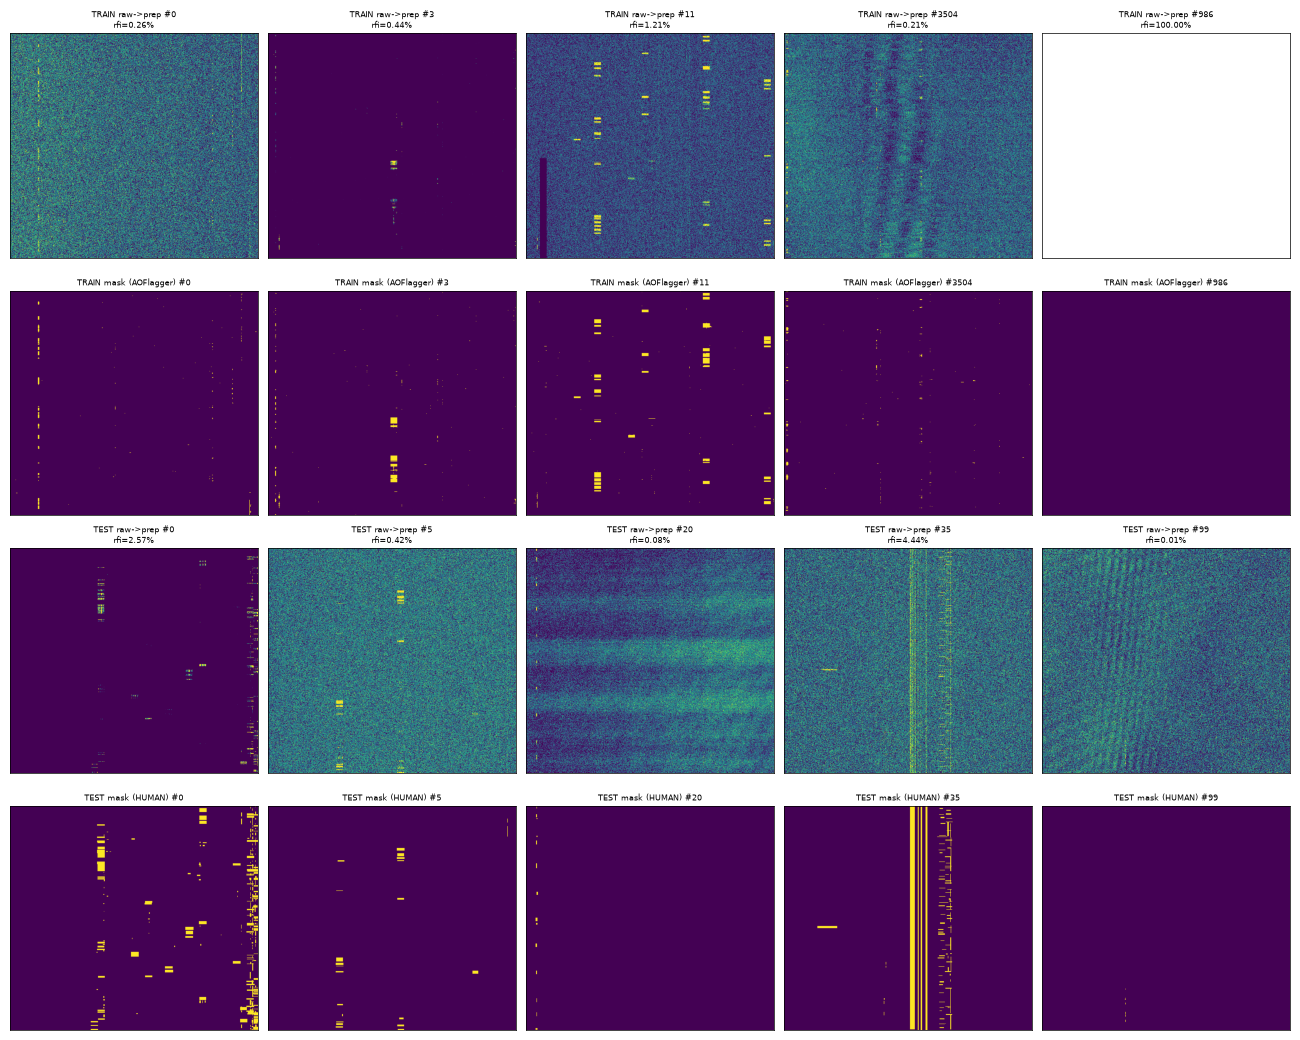
\includegraphics[width=0.85\textwidth]{fig_lofar_overview}
  \caption[Example LOFAR spectrograms and their masks]{Example LOFAR spectrograms (after clipping and log scaling for
    display) and their masks. Top two rows: training images with their
    \aoflagger{} masks; bottom two rows: test images with the human expert's
    masks. Vertical lines are RFI at fixed frequencies.}
  \label{fig:lofar_overview}
\end{figure}

\section{Data Preparation}
\label{sec:lofar_audit}
Before training, two problems in the LOFAR data had to be handled. All 109 test
spectrograms are byte-for-byte identical to 109 of the training spectrograms;
only their masks differ. Training on all 7500 images would therefore test the
model on images it has already seen, so these 109 images were removed from the
training set. In addition, 35 training images are flagged as 100\% RFI, and
several of them contain only zeros, so they were removed as well. This leaves
7356 training images, of which 735 were kept for validation and 6621 used for
training.

The raw LOFAR values are not normalised and range from 0 to
$1.4\times10^{11}$. Every input image $x$ is therefore scaled with one fixed
range for the whole dataset:
\begin{equation}
  x' = \mathrm{clip}\!\left(\frac{x - x_{\text{lo}}}{x_{\text{hi}} - x_{\text{lo}}},\; 0,\; 1\right)
  \label{eq:fixednorm}
\end{equation}
where $x_{\text{lo}}$ and $x_{\text{hi}}$ are the 0.5th and 99.5th percentiles
of the pixel values, averaged over 200 training images (40 for the synthetic
data). Only training images are used, so no information from the test set
enters the normalisation. The reason for using one fixed range rather than
scaling each image separately is explained in \cref{sec:pernorm}.

\section{Baseline Model: \texorpdfstring{\tfunet}{tf\_unet}}
We used the \tfunet{} code of Akeret et al.\ without changing the network
(3 levels, 32 filters in the first layer; \cref{fig:tfunet_arch}). The paper used a batch of 32 images
and momentum gradient descent with a learning rate of 0.2. We used a batch of 4
images, and at such a small batch the paper's learning rate stopped the network
from learning within a few iterations, so we used the Adam optimiser with a
learning rate of $10^{-3}$ instead. On LOFAR the network was trained both with
this setting for 60 epochs and with a learning rate of $10^{-4}$ for 150
epochs.

\begin{figure}[H]
  \centering
  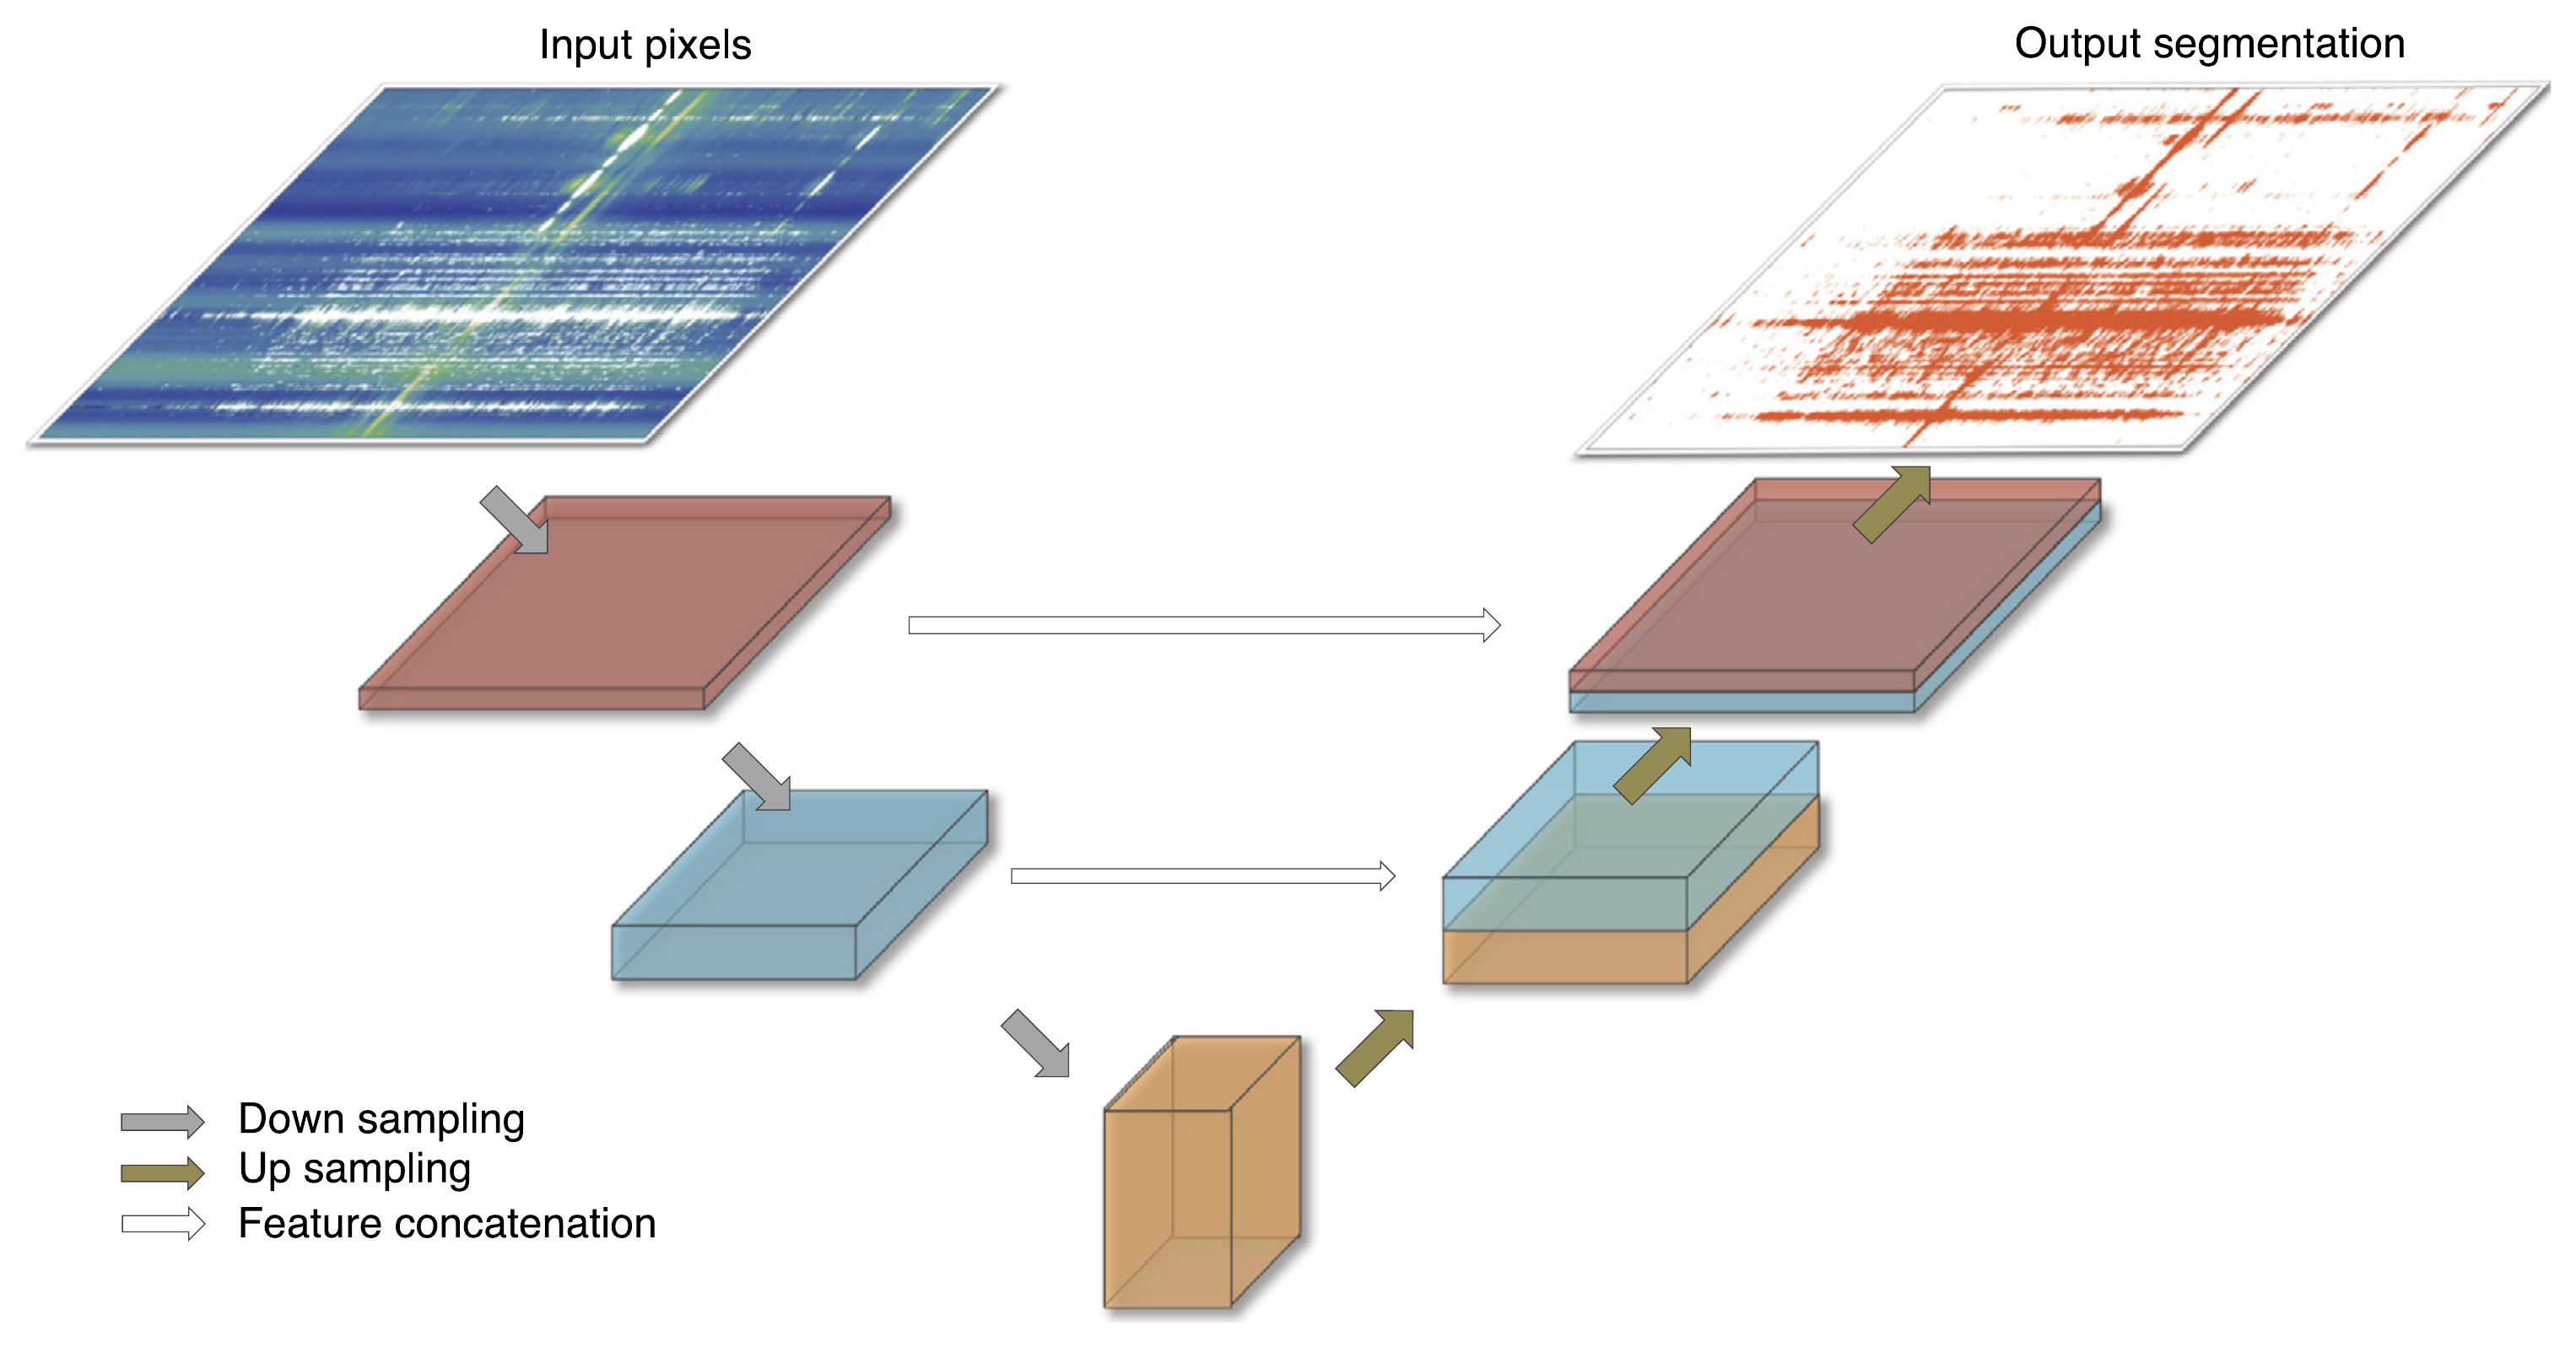
\includegraphics[width=0.85\textwidth]{akeret2017_unet_fig1}
  \caption[The U-Net of \tfunet{} applied to RFI]{The U-Net of \tfunet{}
    applied to RFI, with a depth of 3 levels. The input spectrogram is
    contracted in the downsampling path and expanded again in the upsampling
    path, and features from the downsampling path are concatenated into the
    upsampling path. Reproduced from Akeret et al.\ (2017).}
  \label{fig:tfunet_arch}
\end{figure}

\section{Improved Model: \hybrid{}}
\label{sec:hybrid_design}
\hybrid{} keeps the overall U-Net shape but combines several components that
other RFI and segmentation work has used, chosen with the properties of RFI in
mind. The starting point was that faint RFI sits only about 1.5 noise standard
deviations above the background, so a single pixel cannot be told apart from
noise; a faint line is detectable only because it extends over many pixels.
Most of the design choices aim to use this kind of spatial context.
\Cref{tab:hybrid_vs_tfunet} lists how the model differs from \tfunet{}.

\begin{table}[H]
  \centering
  \caption[Differences between \tfunet{} and \hybrid{}]{Differences between \tfunet{} and \hybrid{}.}
  \label{tab:hybrid_vs_tfunet}
  \small
  \begin{tabular}{>{\raggedright\arraybackslash}p{3.6cm}>{\raggedright\arraybackslash}p{3.9cm}>{\raggedright\arraybackslash}p{5.7cm}}
    \toprule
    Component & \tfunet{} & \hybrid{} \\
    \midrule
    Convolution blocks & two 3$\times$3 convolutions & residual blocks (shortcut through a 1$\times$1 convolution) \\
    Multi-scale filters & none & ``strip'' convolutions, $K = 7, 11, 21$ \\
    Channel attention & none & efficient channel attention (ECA) \\
    Normalisation layers & none & GroupNorm in every residual block and strip module \\
    Output layer & ReLU, then softmax & raw scores, then softmax \\
    Padding & valid (output smaller than input) & same (output = input size) \\
    Times the image is halved / first-layer width & 2 / 32 & 4 / 8 \\
    Loss & cross-entropy & cross-entropy + Dice \\
    Batch size / learning rate on LOFAR & 4 / $10^{-4}$ & 1 / $10^{-3}$ \\
    Framework & TensorFlow & PyTorch \\
    Parameters & 465{,}986 & 593{,}842 \\
    \bottomrule
  \end{tabular}
\end{table}

The components are as follows:
\begin{itemize}
  \item \textbf{Residual blocks}\footcite{he2016} add the input of each block
    back to its output, so that weak features are not washed out as they pass
    through many layers. RFI-Net\footcite{yang2020rfinet}, a published RFI
    network, is also built from residual blocks.
  \item \textbf{Strip convolutions.} Much RFI is line-shaped, and the idea was
    that a long, thin $1\times K$ or $K\times1$ filter adds up the signal along
    such a line: averaging $K$ pixels of a coherent line improves its
    signal-to-noise ratio by about $\sqrt{K}$ (\cref{eq:radiometer}). In the
    implementation, each of the three branches applies a $1\times K$ filter
    followed by a $K\times1$ filter, which together cover a full $K\times K$
    square. Similar multi-scale designs have been used for RFI
    before\footcite{gu2024emsca,mars2026}, so this component is not new.
  \item \textbf{Efficient channel attention} (ECA)\footcite{wang2020eca} learns a
    weight for each feature channel at very little cost, so that channels
    carrying faint RFI are not drowned out by those carrying bright RFI.
  \item \textbf{GroupNorm}\footcite{wu2018groupnorm} keeps the values inside
    the network in a stable range. Unlike batch normalisation, it computes its
    statistics within a single image, so it works with the single-image batches
    used here.
  \item \textbf{No ReLU on the output.} The raw scores go directly to the
    softmax, which avoids the failure of \tfunet{} described in
    \cref{sec:relu_trap}.
  \item \textbf{Same padding} keeps the output the same size as the input, so
    every pixel receives a prediction.
\end{itemize}

\section{Training}
\label{sec:hybrid_training}
\hybrid{} is trained with the sum of the cross-entropy and Dice losses
(\cref{eq:ce,eq:dice}), using the Adam optimiser with a learning rate of
$10^{-3}$ and one image per batch, for 40 epochs of 700 steps (28{,}000
gradient steps). Class weighting, which gives RFI pixels 57 times the weight of
clean ones, was tried first and then removed. For both networks, the best
checkpoint and the decision threshold are chosen on 150 of the 735 validation
images.

\section{Evaluation}
All LOFAR results are measured on the 109 expert-labelled test images, using
the maximum and the pooled \Fone{} (\cref{sec:metrics}). Every setting was
trained with three random seeds, and we report the mean and standard deviation.
To decide whether a difference between two settings is real, we compare them
seed by seed with a paired $t$-test, which with three seeds has 2 degrees of
freedom and needs $|t| > 4.30$ for significance at the 5\% level. To estimate
the uncertainty that comes from the small test set, we also resampled the 109
test images 2000 times with replacement (bootstrap).

\section{Further Experiments}
To understand what drives the performance of \hybrid{}, we carried out four
further experiments:
\begin{itemize}
  \item \textbf{Ablation.} We wrote a version of the network in which each
    component can be switched off, and trained every variant through exactly
    the same pipeline, removing the strip convolutions, the attention, the
    residual blocks, all three together, and finally also GroupNorm.
  \item \textbf{CRF refinement.} Chen et al.\footcite{chen2023} refine RFI
    labels with a conditional random field (CRF)\footcite{krahenbuhl2011}, which
    adjusts each pixel's label according to its neighbours. Following them, we
    added a CRF on top of the trained network. It was implemented as
    differentiable layers\footcite{zheng2015crfrnn,teichmann2018convcrf}, so
    that its settings can be set by hand or learned, with separate ranges along
    time and frequency. It adds only 11 parameters.
  \item \textbf{Expert labels.} To measure what expert labels add without ever
    testing on an image whose expert label the model has seen, we used
    five-fold cross-validation over the 109 expert-labelled images, keeping
    near-duplicate images in the same fold. In each fold 21--22 images form the
    test set, 19 the validation set and the remaining 68--69 can be used for
    fine-tuning, with a learning rate of $10^{-4}$. We also labelled only 5, 10
    or 20\% of them, as $64\times64$ patches chosen by the model's uncertainty,
    by its predicted RFI, or at random, or as whole images chosen at random.
  \item \textbf{Loss.} We trained \hybrid{} again with plain cross-entropy
    instead of cross-entropy plus Dice, keeping everything else the same.
\end{itemize}
